% In this section, the layer is described in some detail in terms of its specific subsystems. Describe each of the layers and its subsystems in a separate chapter/major subsection of this document. The content of each subsystem description should be similar. Include in this section any special considerations and/or trade-offs considered for the approach you have chosen.
The Firebase layer consists of three subsystems, Firebase Firestore Database, Firebase Authentication, and Firebase Service.

\begin{figure}[h!]
    \centering
    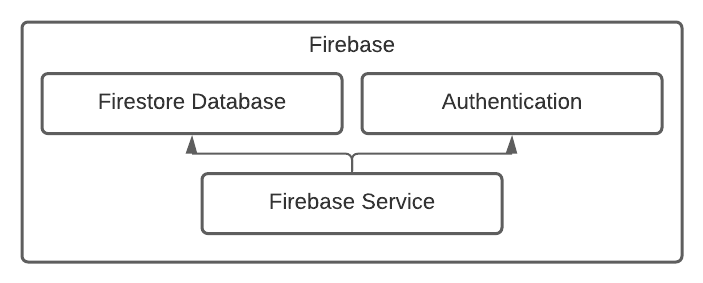
\includegraphics[width=0.60\textwidth]{images/ADS_Diagram_Firebase}
    \caption{Firebase layer diagram}
\end{figure}

\subsection{Firebase Firestore Database}
%  This section should be a general description of a particular subsystem for the given layer. For most subsystems, an extract of the architectural block diagram with data flows is useful. This should consist of the subsystem being described and those subsystems with which it communicates.

Firebase Firestore Database is hosted by Google and it holds the data for all users and all of the courses.
The data is provided to the website upon request by users.

\subsubsection{Assumptions}
%  Any assumptions made in the definition of the subsystem should be listed and described. Pay particular attention to assumptions concerning interfaces and interactions with other layers.
\begin{itemize}
    \begin{item}
          Exceptions will be handled by the calling subsystems.
    \end{item}
    \begin{item}
          The user must have Internet connection
    \end{item}
    \begin{item}
          The subsytem should not be used directly by any other subsystem except for Firebase Service
    \end{item}
\end{itemize}

\subsubsection{Responsibilities}
% Each of the responsibilities/features/functions/services of the subsystem as identified in the architectural summary must be expanded to more detailed responsibilities. These responsibilities form the basis for the identification of the finer-grained responsibilities of the layer's internal subsystems. Clearly describe what each subsystem does.
\begin{itemize}
    \begin{item}
          Storing the course catalog
    \end{item}
    \begin{item}
          Storing the user's data, including their user ID, major, starting semester, and chosen courses
    \end{item}
\end{itemize}

\subsubsection{Subsystem Interfaces}
%  Each of the inputs and outputs for the subsystem are defined here. Create a table with an entry for each labelled interface that connects to this subsystem. For each entry, describe any incoming and outgoing data elements will pass through this interface.
\begin {table}[H]
\caption {Firebase Firestore Database Subsystem interfaces}
\begin{center}
    \begin{tabular}{ | p{1cm} | p{6cm} | p{3cm} | p{3cm} |}
        \hline
        ID  & Description       & Inputs       & Outputs                   \\ \hline
        \#1 & Get Courses       & \pbox{3cm}{} & \pbox{3cm}{Courses}       \\ \hline
        \#2 & Get Courses Taken & \pbox{3cm}{} & \pbox{3cm}{Courses Taken} \\ \hline
    \end{tabular}
\end{center}
\end{table}




\subsection{Firebase Authentication}
%  This section should be a general description of a particular subsystem for the given layer. For most subsystems, an extract of the architectural block diagram with data flows is useful. This should consist of the subsystem being described and those subsystems with which it communicates.

Firebase Authentication is hosted by Google and it handles authenticating the users before they can use the website.
A user will be authenticated when the correct credentials are provided, or a new account is created.

\subsubsection{Assumptions}
%  Any assumptions made in the definition of the subsystem should be listed and described. Pay particular attention to assumptions concerning interfaces and interactions with other layers.
\begin{itemize}
    \begin{item}
          Exceptions will be handled by the calling subsystems.
    \end{item}
    \begin{item}
          The user must have Internet connection
    \end{item}
    \begin{item}
          The subsytem should not be used directly by any other subsystem except for Firebase Service
    \end{item}
\end{itemize}

\subsubsection{Responsibilities}
% Each of the responsibilities/features/functions/services of the subsystem as identified in the architectural summary must be expanded to more detailed responsibilities. These responsibilities form the basis for the identification of the finer-grained responsibilities of the layer's internal subsystems. Clearly describe what each subsystem does.
\begin{itemize}
    \begin{item}
          Authenticating users so only logged in users can access the degree planner.
    \end{item}
    \begin{item}
          Logging out users
    \end{item}
    \begin{item}
          Changing password
    \end{item}
\end{itemize}

\subsubsection{Subsystem Interfaces}
%  Each of the inputs and outputs for the subsystem are defined here. Create a table with an entry for each labelled interface that connects to this subsystem. For each entry, describe any incoming and outgoing data elements will pass through this interface.
\begin {table}[H]
\caption {Firebase Authentication Subsystem interfaces}
\begin{center}
    \begin{tabular}{ | p{1cm} | p{6cm} | p{3cm} | p{3cm} |}
        \hline
        ID  & Description     & Inputs              & Outputs                \\ \hline
        \#1 & Log in          & \pbox{3cm}{Email                             \\ Password} & \pbox{3cm}{User Object}  \\ \hline
        \#2 & Sign up         & \pbox{3cm}{Username                          \\ Email \\ Password}  & \pbox{3cm}{User Object} \\ \hline
        \#3 & Logout          & \pbox{3cm}{}        & \pbox{3cm}{Success}    \\ \hline
        \#4 & Change Password & \pbox{3cm}{Email}   & \pbox{3cm}{Email Sent} \\ \hline
    \end{tabular}
\end{center}
\end{table}




\subsection{Firebase Service}
%  This section should be a general description of a particular subsystem for the given layer. For most subsystems, an extract of the architectural block diagram with data flows is useful. This should consist of the subsystem being described and those subsystems with which it communicates.

The next subsystem is Firebase Serivice. This subsystem is programmed in the website and controls how 
the website interacts with the Firebase Database Subsystem and Firebase Authentication.

\subsubsection{Assumptions}
%  Any assumptions made in the definition of the subsystem should be listed and described. Pay particular attention to assumptions concerning interfaces and interactions with other layers.
\begin{itemize}
    \begin{item}
          Exceptions will be handled, and rethrown is neccessary.
    \end{item}
    \begin{item}
          The user must have Internet connection
    \end{item}
    \begin{item}
          The subsytem should be the only subsystem to access Firebase Firestore Database and Firebase Authentication
    \end{item}
\end{itemize}

\subsubsection{Responsibilities}
% Each of the responsibilities/features/functions/services of the subsystem as identified in the architectural summary must be expanded to more detailed responsibilities. These responsibilities form the basis for the identification of the finer-grained responsibilities of the layer's internal subsystems. Clearly describe what each subsystem does.
\begin{itemize}
    \begin{item}
          Control all interactions with Firebase Firestore Database and Firebase Authentication to reduce code duplication
    \end{item}
    \begin{item}
          Authenicating users
    \end{item}
    \begin{item}
          Log out user
    \end{item}
    \begin{item}
          Changing password
    \end{item}
    \begin{item}
          Update user data
    \end{item}
    \begin{item}
          Retrieve all courses
    \end{item}
\end{itemize}

\subsubsection{Subsystem Interfaces}
%  Each of the inputs and outputs for the subsystem are defined here. Create a table with an entry for each labelled interface that connects to this subsystem. For each entry, describe any incoming and outgoing data elements will pass through this interface.
\begin {table}[H]
\caption {Firebase Service Subsystem interfaces}
\begin{center}
    \begin{tabular}{ | p{1cm} | p{6cm} | p{3cm} | p{3cm} |}
        \hline
        ID   & Description           & Inputs                        & Outputs                \\ \hline
        \#1  & Log in                & \pbox{3cm}{Email                                       \\ Password} & \pbox{3cm}{User Object}  \\ \hline
        \#2  & Sign up               & \pbox{3cm}{Username                                    \\ Email \\ Password}  & \pbox{3cm}{User Object} \\ \hline
        \#3  & Logout                & \pbox{3cm}{}                  & \pbox{3cm}{Success}    \\ \hline
        \#4  & Forgot Password       & \pbox{3cm}{Email}             & \pbox{3cm}{Email Sent} \\ \hline
        \#5  & Get Courses           & \pbox{3cm}{}                  & \pbox{3cm}{Courses}    \\ \hline
        \#6  & Set Major             & \pbox{3cm}{Major}             & \pbox{3cm}{Success}    \\ \hline
        \#7  & Set Starting Semester & \pbox{3cm}{Starting Semester} & \pbox{3cm}{Success}    \\ \hline
        \#8  & Add Chosen Course     & \pbox{3cm}{Semester                                    \\ Course ID} & \pbox{3cm}{Success}    \\ \hline
        \#9  & Remove Chosen Course  & \pbox{3cm}{Semester                                    \\ Course ID} & \pbox{3cm}{Success}    \\ \hline
        \#10 & Get Chosen Courses    & \pbox{3cm}{}                  & \pbox{3cm}{Courses}    \\ \hline
    \end{tabular}
\end{center}
\end{table}
